\begin{frame}{Validation of 2D Axisymmetric model:Two-Phase Steam Ejector}
    \begin{figure}
        \centering
        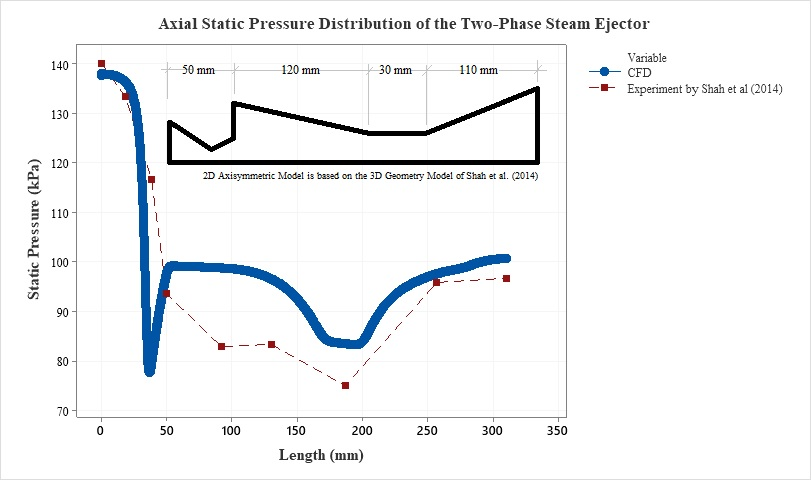
\includegraphics[height=5.25cm]{images/ValidationPressureProfile.jpg}
        \label{fig:shahexperimental}
    \end{figure}
\end{frame}

\begin{frame}{Two-Phase Steam Ejector}
    \begin{columns}
  \column{0.45\textwidth}
    \begin{figure}
        \centering
        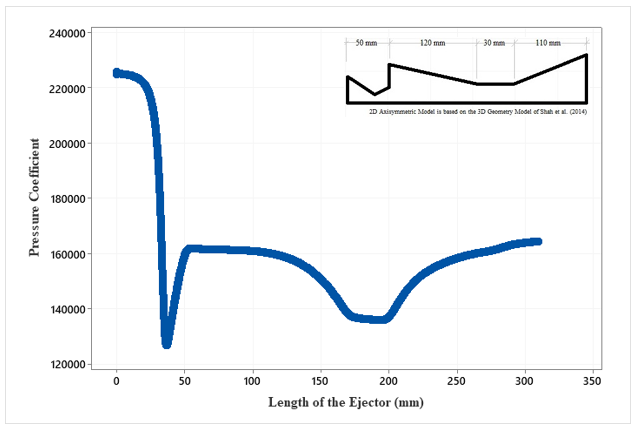
\includegraphics[height=4.5cm]{images/tpseprescoef.png}
    \end{figure}
  \column{0.45\textwidth}
  \begin{figure}
        \centering
        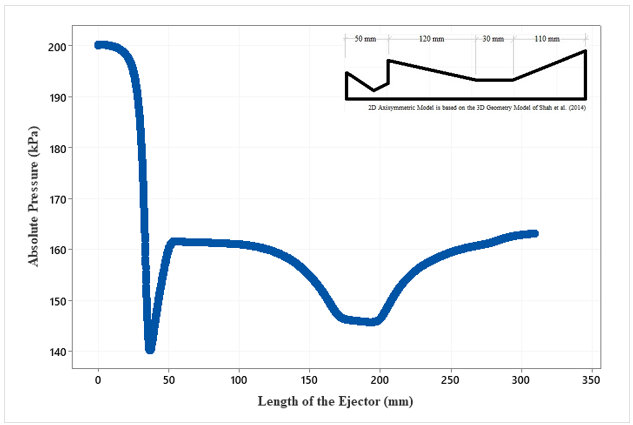
\includegraphics[height=4.5cm]{images/tpseabspres.png}
    \end{figure}
 \end{columns}
\end{frame}

\begin{frame}{Two-Phase Steam Ejector}
    \begin{columns}
  \column{0.45\textwidth}
    \begin{figure}
        \centering
        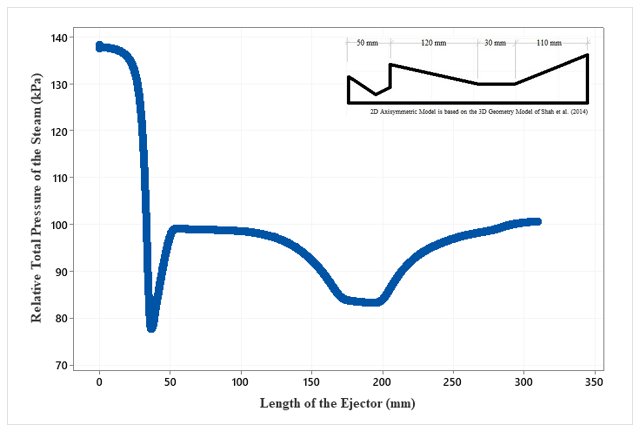
\includegraphics[height=4.5cm]{images/tpseRTPsteam.png}
    \end{figure}
  \column{0.45\textwidth}
  \begin{figure}
        \centering
        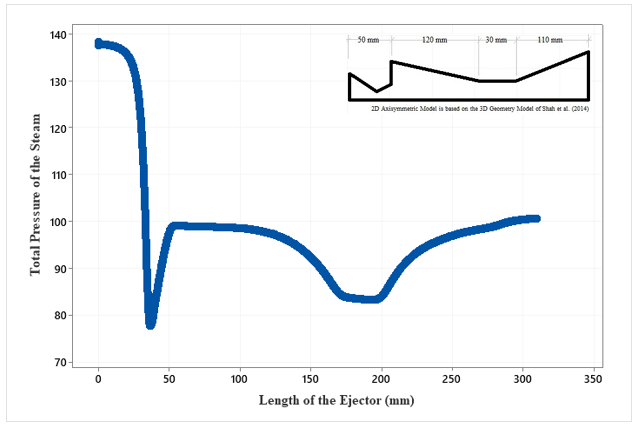
\includegraphics[height=4.5cm]{images/tpsetpsteam.png}
    \end{figure}
 \end{columns}
\end{frame}

\begin{frame}{Two-Phase Steam Ejector}
    \begin{columns}
  \column{0.45\textwidth}
    \begin{figure}
        \centering
        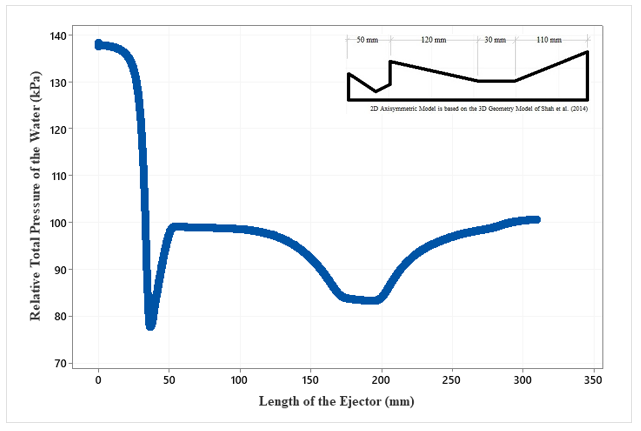
\includegraphics[height=4.5cm]{images/tpsertpwater.png}
    \end{figure}
  \column{0.45\textwidth}
  \begin{figure}
        \centering
        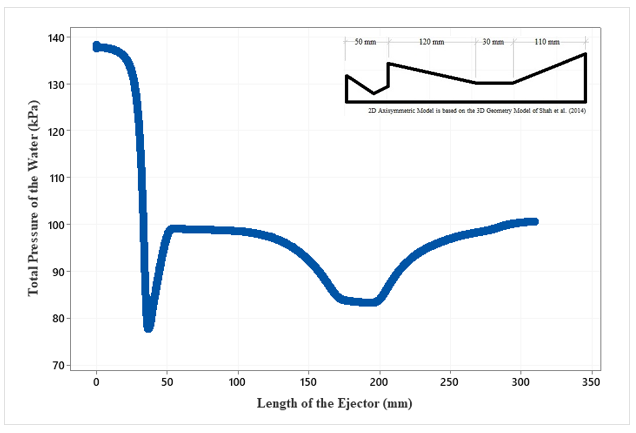
\includegraphics[height=4.5cm]{images/tpsetpwater.png}
    \end{figure}
 \end{columns}
\end{frame}

\begin{frame}{Validation of 2D Axisymmetric model: Two-Phase CO2 Converging-Diverging Nozzle: Mixture of CO2 and Air}
 \begin{columns}
  \column{0.45\textwidth}
    \begin{figure}
        \centering
        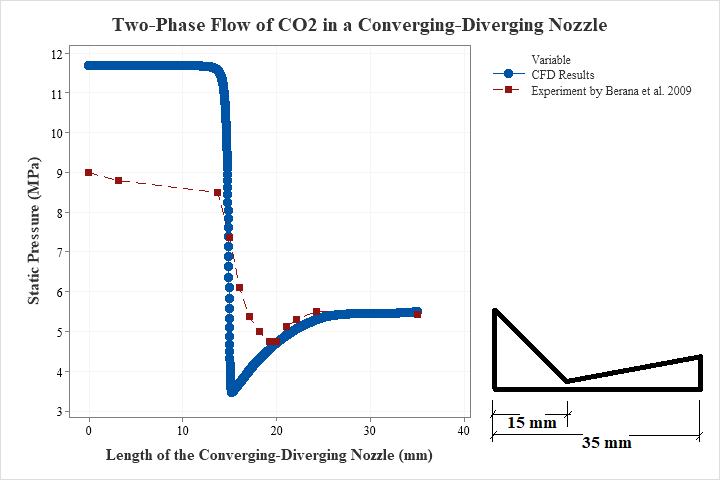
\includegraphics[height=4.5cm]{images/co2718secresult.png}
        \caption{Time Step of 0.000718 sec}
    \end{figure}
  \column{0.45\textwidth}
  \begin{figure}
        \centering
        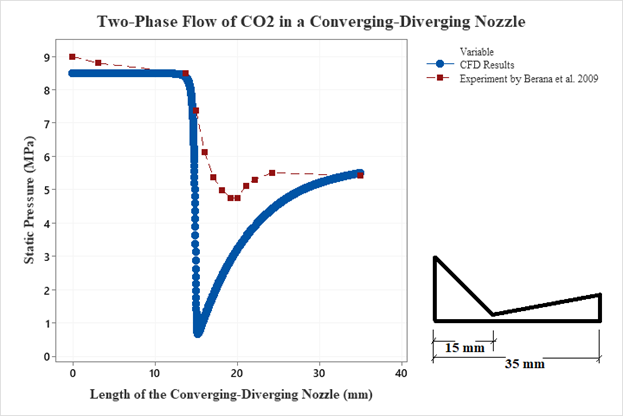
\includegraphics[height=4.5cm]{images/co2at135sec.png}
        \caption{Time Step of 0.00113 sec (Steady Operation)}
    \end{figure}
 \end{columns}
\end{frame}

\begin{frame}{Validation of 2D Axisymmetric model: Two-Phase CO2 Converging-Diverging Nozzle:Air and CO2}
 \begin{columns}
  \column{0.45\textwidth}
    \begin{figure}
        \centering
        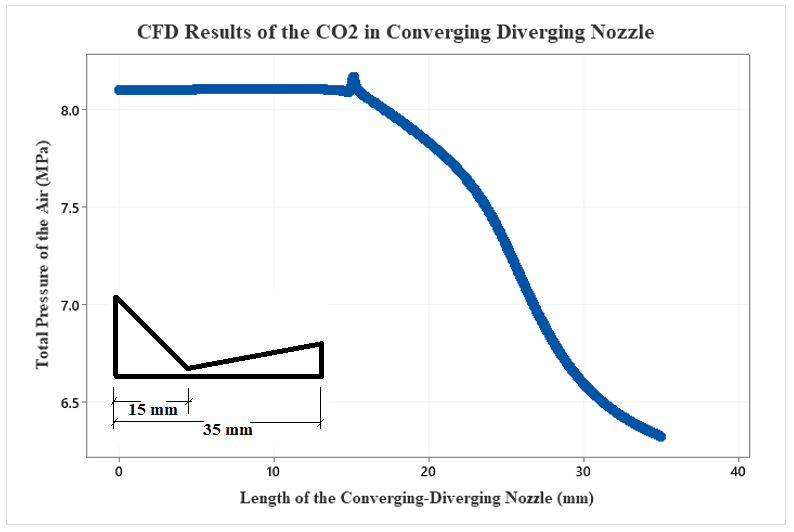
\includegraphics[height=4.5cm]{images/cdnco2totalpress.png}
    \end{figure}
  \column{0.45\textwidth}
  \begin{figure}
        \centering
        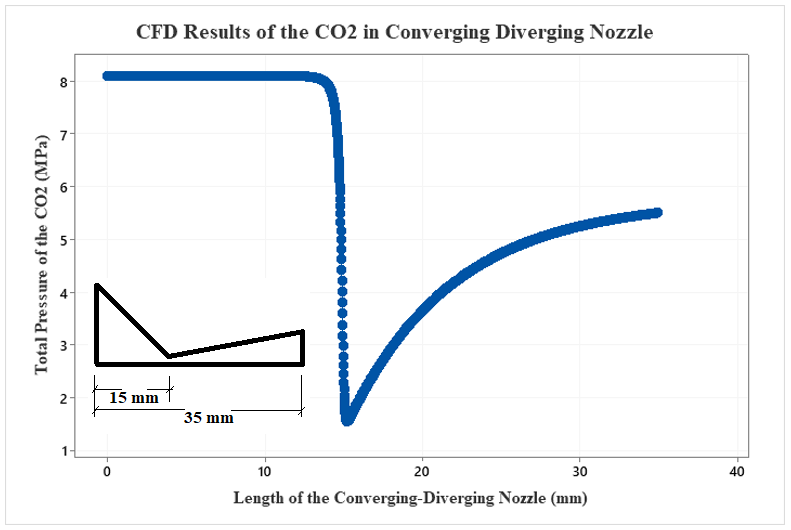
\includegraphics[height=4.5cm]{images/cdnco2press1.png}
    \end{figure}
 \end{columns}
\end{frame}

\begin{frame}{Validation of 2D Axisymmetric model: Two-Phase CO2 Converging-Diverging Nozzle:Air and CO2}
 \begin{columns}
  \column{0.45\textwidth}
    \begin{figure}
        \centering
        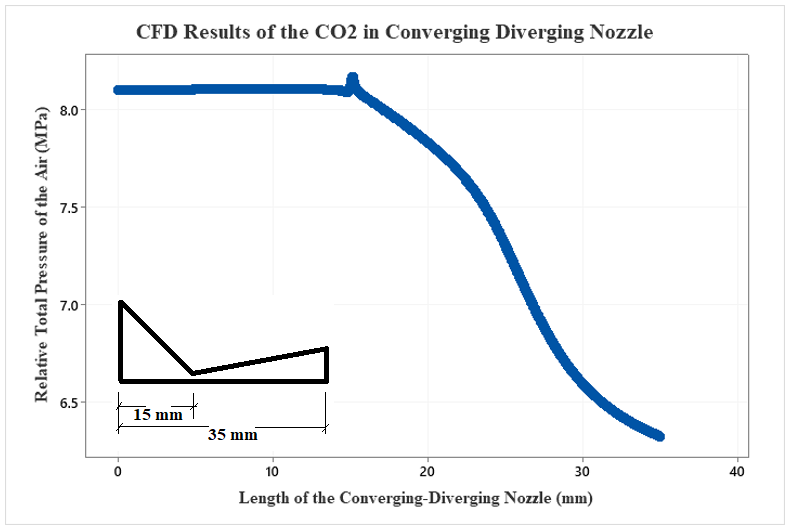
\includegraphics[height=4.5cm]{images/cdnrelativepress1.png}
    \end{figure}
  \column{0.45\textwidth}
  \begin{figure}
        \centering
        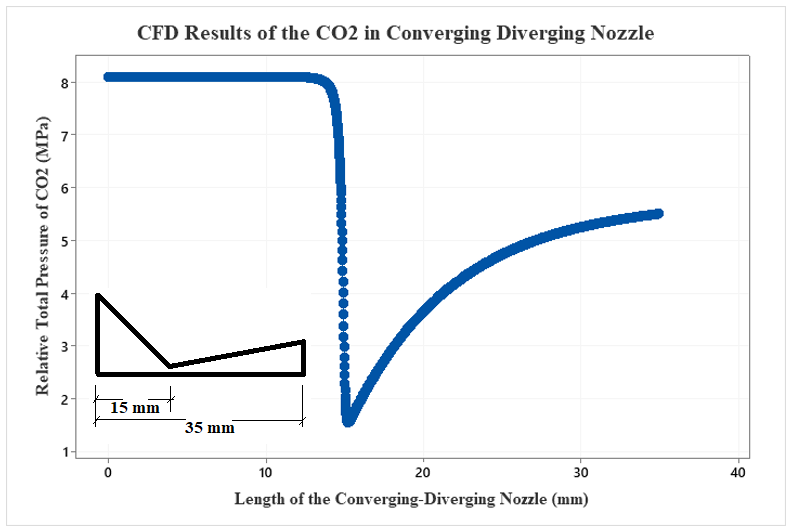
\includegraphics[height=4.5cm]{images/cdnrelativepress2.png}
    \end{figure}
 \end{columns}
\end{frame}

\begin{frame}{Validation of 2D Axisymmetric model: Two-Phase CO2 Converging-Diverging Nozzle: Air and CO2}
 \begin{columns}
  \column{0.45\textwidth}
    \begin{figure}
        \centering
        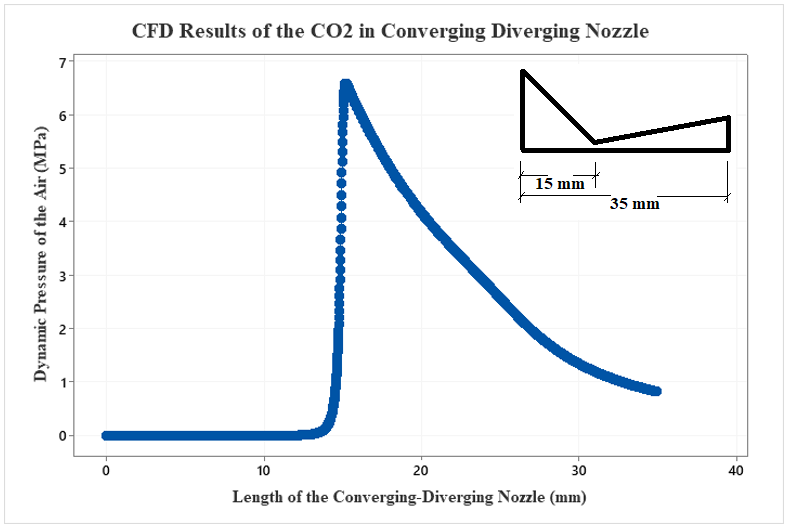
\includegraphics[height=4.5cm]{images/co2dynamicpressair.png}
    \end{figure}
  \column{0.45\textwidth}
  \begin{figure}
        \centering
        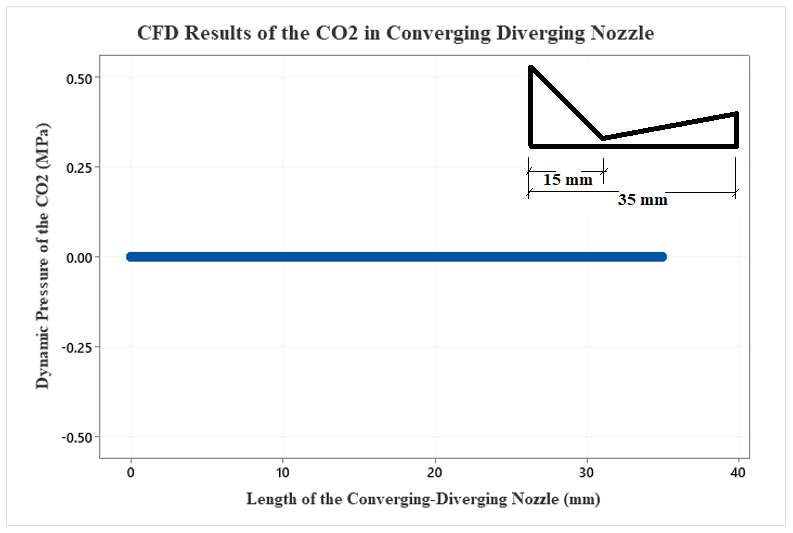
\includegraphics[height=4.5cm]{images/co2dynamicpres.png}
    \end{figure}
 \end{columns}
\end{frame}